% P41 Figure: Minkowski directions and three CMCA layers
\begin{figure}[htbp]
\centering
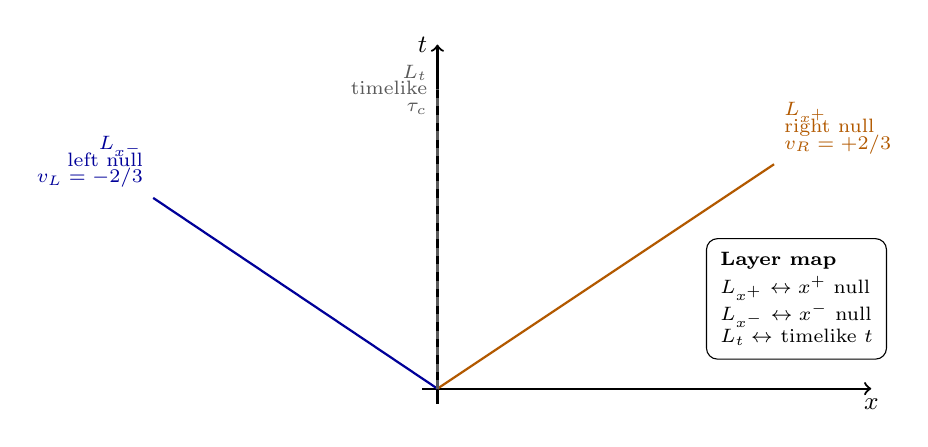
\begin{tikzpicture}[scale=0.95, every node/.style={font=\small}]
  % Axes
  \draw[->,thick] (-0.2,0) -- (5.8,0) node[below] {$x$};
  \draw[->,thick] (0,-0.2) -- (0,4.6) node[left] {$t$};
  % Light cone rays (lattice speeds ±2/3 shown schematically)
  \draw[thick,orange!70!black] (0,0) -- (4.5,3.0)
    node[above right,font=\scriptsize,align=left] {$L_{x^+}$\\[-2pt]right null\\[-2pt]$v_R=+2/3$};
  \draw[thick,blue!60!black] (0,0) -- (-3.8,2.55)
    node[above left,font=\scriptsize,align=right] {$L_{x^-}$\\[-2pt]left null\\[-2pt]$v_L=-2/3$};
  \draw[thick,gray!70!black,dashed] (0,0) -- (0,4.0)
    node[left,font=\scriptsize,align=right] {$L_t$\\[-2pt]timelike\\[-2pt]$\tau_c$};
  % Layer correspondence box
  \node[draw,rounded corners,fill=white,align=left,font=\scriptsize,inner sep=5pt]
    at (4.8,1.2) {
    \textbf{Layer map}\\[2pt]
    $L_{x^+}\leftrightarrow x^+$ null\\
    $L_{x^-}\leftrightarrow x^-$ null\\
    $L_t\leftrightarrow$ timelike $t$
  };
\end{tikzpicture}
\caption{The three CMCA layers exhaust the irreducible causal directions of
  $1{+}1$D Minkowski spacetime: two null (chiral) layers plus one timelike
  gating layer. Glider speeds $|v_R|=|v_L|=2/3$ restore the discrete light cone.}
\label{fig:minkowski_cmca_map}
\end{figure}
